\documentclass[10pt,a4paper]{article}
\usepackage[utf8]{inputenc}
\usepackage[parfill]{parskip}
\usepackage[section]{placeins}
\usepackage{graphicx}
\usepackage{array}
\usepackage{tikz}
\usepackage{apacite}
\usepackage{url}

\title{\Huge{Sentiment Analysis for Social Media Comments}}
\author{Christoph Emunds, Benedikt Heinrichs, Dominik Nerger, Richard Polzin}
\date{\today}

\begin{document}
	\pagenumbering{gobble}
	
	\maketitle
	\begin{abstract}
	Analyzing customer experience offers valuable data for Business Intelligence. Especially in e-commerce, where users write reviews about products and services, the analysis of the customers' sentiment towards these entities yields significant insights into potential strengths and weaknesses of the product or service.

	Our work focuses on evaluating customer experience through the application of aspect-based sentiment analysis on social media posts. The data set contains a year's worth of Facebook comments on the pages of the two supermarket chains Tesco and Sainsbury. The goal is to extract as many triplets $(e, a, s)$ as possible, where $e$ is an entity (product or service), $a$ is an aspect of this entity (performance, battery, politeness, etc.), and $s$ is the sentiment polarity label (negative, neutral, positive).

	To accomplish this task, many different subtasks need to be solved. After a rudimentary preprocessing routine, the posts need to be identify the part of speech (POS) category for every word. Then Named Entity Recognition (NER) must be applied and words containing sentiment need to be detected and evaluated. As a significant number of social media texts do not follow the grammatical rules or contain a lot of misspellings the complexity of those tasks is increased significantly. With the completed analysis we identify potential products and services, their corresponding aspects and sentiment words, which are scored and aggregated into opinions.

	The results obtained from this analysis are visualized to get a better understanding of the customers' feelings towards these products, services, and their aspects. The visualization supports businesses in a wide range of decisions, such as product positioning and pricing. This can lead to better customer satisfaction, faster reactions to trends and overall revenue growth.
	\end{abstract}
	
	\newpage
	\tableofcontents
	\newpage
	
	\pagenumbering{arabic}
	\section{Introduction}
	% What is sentiment analysis?
	% What does "aspect-based" mean?
	% What do we show?
	
	Sentiment analysis or opinion mining uses techniques from natural language processing (NLP), text analysis, and computational linguistics to extract subjective information from texts. In applications that involve analyzing customer experience, this subjective information typically represents the position of a person towards a certain entity. Quantifying feelings and opinions that customers have towards products and services offers valuable information for the company.
	
	% Copied from websites, needs rephrasing
	%In this context, Aspect Based Sentiment Analysis (ABSA) - i.e., mining and summarizing opinions from text about specific entities and their aspects - can help consumers decide what to purchase and businesses to better monitor their reputation and understand the needs of the market.
	%Sentiment analysis is increasingly viewed as a vital task both from an academic and a commercial standpoints. The majority of current approaches, however, attempts to detect the overall polarity of a sentence, paragraph, or text span, regardless of the entities mentioned (e.g., laptops, restaurants) and their aspects (e.g., battery, screen; food, service). By contrast, this task is concerned with aspect based sentiment analysis, where the goal is to identify the aspects of given target entities and the sentiment expressed towards each aspect.
	
	The project presented in this document focuses on finding and analyzing customers' opinions on products and their aspects from social media posts of a supermarket chain. In today's world, social media is a big part of the social life. On social networks like Facebook, besides personal accounts there are corporate accounts as well, with the possibility of people interacting with e.g. companies, celebrities, or sports teams. People can review companies or comment on their news feed. These comments or reviews are often filled with positive or negative sentiments, since they mostly occur after a really positive or negative experience with the company. Through the comments, it should therefore be possible to extract sentiments about products or aspects of the company.
		
	\section{Related work}
	The related work presented in this section should give a quick overview over two of the main techniques that we used to identify entities and their aspects.
		
		\subsection{POS-Tagging}		
		POS-Tagging (part-of-speech tagging), also called grammatical tagging or word-category disambiguation, refers to the process of identifying particular parts of speech like nouns or verbs. Identifying the role of a certain word within a sentence is important for the task of sentiment analysis, as identifying entities and their corresponding aspects can be handled much easier relying on certain assumptions about the part of speech of words.
		
		While being important POS-Tagging is also a complex problem. Word-forms in natural language are often ambiguous. For example the word 'dogs' is usually thought of as a plural noun, but can be used as a verb as well:

		\begin{quote}
			The sailor dogs the hatch.
		\end{quote}

		Due to the complexity, machine learning techniques are often applied in POS-Taggers. Popular approaches such as the Viterbi algorithm, the Brill tagger or the Baum-Welch algorithm work with techniques such as dynamic programming, supervised learning or hidden Markov models.
		
		\subsection{NER-Tagging}
		
		Named-Entity recognition (NER) is a task that seeks to locate and classify specific information in text. This information is called a named entity and can refer to categories such as the names of persons, locations, times or many others.

		An annotated sentence could look like this :

		\begin{quote}
			[Tim Cook]$_{[Person]}$ has a Net worth of [785 million USD]$_{[Monetary Value]}$ as of [March 16. 2017]$_{[Time]}$.
		\end{quote}
		
		While state-of-the-art NER-Taggers perform very well and produce near-human performance they are also brittle and do not perform well in domains they were not designed for.
	
	\section{Approach}
	% Which steps are necessary?

		\subsection{Preprocessing}
		We pre-processed the data by extracting the actual text of the posts into separate files. We decided to exclude posts that are less than 20 characters long or include images. This is due to the fact that posts which are too short do not yield much information most of the time. Furthermore, posts that include images often refer to objects in the image, which makes it hard to understand the author's sentiment without analyzing the image content.
	
		\subsection{Extracting entities and aspects}
		\label{sec:entityextraction}
		POS-tagging and Named Entity Extraction with OpenNLP
		
		Because no pre-trained model exists for the Named Entity Recognition of products or services, we decided to use the OpenNLP model for organizations. Because most nouns in the English language are written in lower case, but organizations as well as products contain capital letters, the OpenNLP model for organizations is a fitting alternative to bypass the non-existent models for products and services. Therefore, we consider everything that is tagged as \textit{Organization} as a product or service.
		% Uses maximum entropy?
		% Mainly Dominik's part

		Searching for aspects is done by iterating over the complete set of posts for each entity. If a post contains the product, we identify the sentences it appears in. We then look for other nouns in these sentences and count their frequency. From those potential aspects, we consider the ones to be real aspects that occur at least in 10\% of the posts that mentioned the product.

		After identifying a set of aspects for each entity, we merge similar entities and their aspect lists by tokenizing the entities' names and lemmatizing them. This results in a reduction of entities, e.g. \textit{Customer Service} and \textit{Customer Services} are considered as the same entity. The entities' aspect lists are merged accordingly. All aspects that are also part of the entity's name are removed from the aspect list. Amongst other things, this removes the aspects \textit{tesco} and \textit{express} from the list of aspects for the entity \textit{Tesco Express}.

		If no aspects can be found for a specific entity, it is removed from the final list of entities.
		For every entity that is part of the final list, the aspect \textit{general} is added as well.

		\subsection{Determining sentiment polarities}
		nltk's Vader module
		Specifically developed for social media

	\section{Results}
	\label{sec:results}
	% len(posts) = 37701
	% len(preprocessed_posts) = 22395
	
	% len(products_original) = 1598
	% len(products) = 1379 (after removing some by hand)
	% len(products_and_aspects) = 1256
	
	We were given a data set containing a year's worth of Facebook comments on the pages of two supermarket chains Tesco and Sainsbury. However, we decided to perform our approach only on the Tesco data set.

	The original goal was to extract as many quintuples $(e_i, a_{ij}, s_{ijkl}, h_k, t_l)$ as possible, where $e_i$ is the $i$'th entity and $a_{ij}$ is the $j$'th aspect of entity $i$ the opinion is expressed on. $s_{ijkl}$ is the sentiment polarity, which can take on the values \textit{positive} or \textit{negative}. $h_k$ describes the opinion holder and $t_l$ the time at which the opinion was expressed.

	However, from the data set that was given to us, it was not possible to determine the person that wrote a post. Moreover, we did not focus on extracting the time a certain sentiment was expressed, as we did not aim to provide a temporal overview over the shifting of opinions towards the products and services.

	We labeled a small subset of posts concerning the entity \textit{Customer Service} by hand. This includes 200 posts with 254 extracted sentiment triples with unknown sentiment.

	After labeling these triples with the Vader module, 139 of the 254 triples (i.e. 54.72\%) result in the same sentiment.

		\subsection{Visualization}
		We will use the sentiment lexicon by \cite{Hu:2004:MSC:1014052.1014073}, which includes mis-spellings, morphological variants, slang and social-media mark-up of 2006 positive and 4783 negative words.

		On the server side, we use Python with the library Flask. On the client side, we use the JavaScript libraries d3.js, vue.js and jQuery.
	
		For the visualization, we use the \textit{JSON} file containing the aggregated opinions that are the result of executing the pipeline as well as a \textit{JSON} containing the positive and negative sentiment words that are provided by the lexicon-based sentiment analysis.
	
		The data is visualized with each product having its own page that is loaded from a dropdown menu and each aspect of the product being visualized with a bar chart as well as the specific posts being shown below the bar chart. The bar chart can be seen in Figure \ref{fig:barchart}. It shows the amount of negative, neutral and positive sentiments regarding the combination of product and aspect.
	
		\begin{figure}[h]
			\centering
			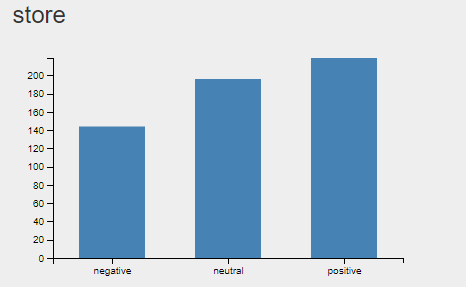
\includegraphics[width=0.7\linewidth]{data/barchart}
			\caption{Bar chart displaying the sentiments regarding the customer service with aspect 'store'}
			\label{fig:barchart}
		\end{figure}
			
		An excerpt of posts regarding the combination of product and aspect is shown below each bar chart, with a maximum of 10 posts per aspect. In Figure \ref{fig:posts}, the highlighted posts can be seen. Positive and negative sentiments are highlighted in colors green and red, respectively. Mentions of the product are highlighted in orange and the aspect is shown with a cyan highlighting.
			
		\begin{figure}[h]
			\centering
			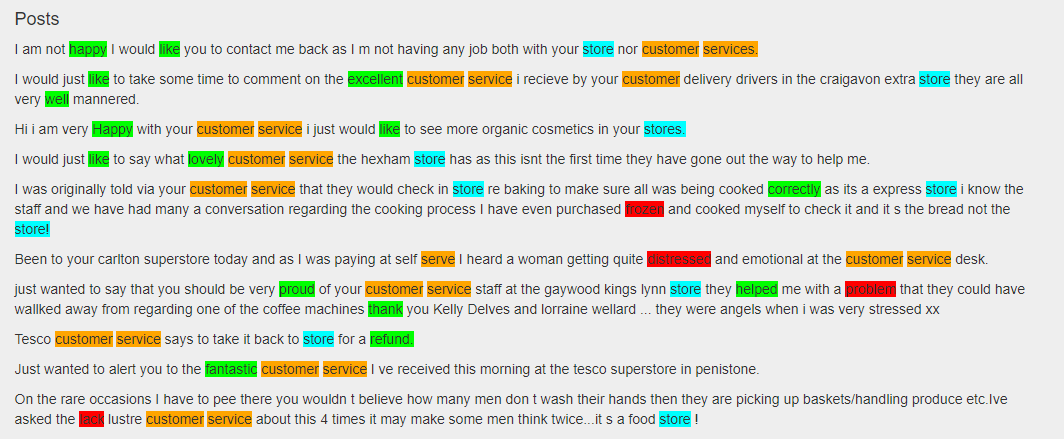
\includegraphics[width=0.9\linewidth]{data/posts}
			\caption{Highlighted posts regarding the customer service with aspect 'store'}
			\label{fig:posts}
		\end{figure}
	
	\section{Discussion and Conclusion}
	The accuracy of 54.72\% as mentioned in Section \ref{sec:results} leaves a lot of potential for improvement. Several factors contribute to this rather bad accuracy score. First of all, the 200 posts that were labeled by hand are by no means indicative of the actual data set. Furthermore, we did not test different target functions for the polarity determination. Due to the lack of time, each of the four contributors tagged 50 posts. There is no guarantee that two people agree with what the other person labeled (would need Kappa measure).

	We do not account for multi token aspects, since we only identify common nouns, which are single words.

	Like mentioned in Section \ref{sec:entityextraction}, we consider every organization found as product or service. This has many caveats. For one, it is required that services like \textit{Customer Service} actually appear capitalized in our data set at least once to be found. Moreover, a lot of things that are not actually organizations are tagged as such. This could be improved by incorporating more knowledge regarding common nouns and noun phrases.
	% Furthermore we take absolutely every "organization" into account and do use a frequency threshold, which might clean up the result a lot
	Moreover, the results could be improved by finding a model that has been trained on products, which would result in more accurate entities and aspects.
	%We use the sentiment of the whole sentence to determine the sentiment towards the aspect
	
	\section{Appendix}
	%TODO: Make proper appendix, don't know the commands from the top of my head
		
		\subsection{Using the code}
		To reproduce our work, the provided code has to be executed in a certain sequence. The following will talk about the needed steps.

	\newpage

	\bibliography{rp}
	\bibliographystyle{apacite}
\end{document}